\section{Results}\label{sec:results}

In order to test the \code{aneris} harmonization procedure, results from the IAM
MESSAGE-GLOBIOM \cite{fricko_marker_2017} was processed. Two scenarios from the
SSP scenario library \cite{Riahi2017153,Rao2017346} are investigated. The SSP2,
or ``middle of the road'', scenario family is chosen to be analyzed because
MESSAGE-GLOBIOM is the marker scenario for this SSP. Of all SSP2 scenarios, the
reference (marker) and SSP2-45 scenarios are analyzed. Notably, emissions from
multiple sectors tend to increase in the reference scenario, thus testing the
harmonization mechanism with an increasing emissions pathway. The SSP2-45
scenario, where the ``45'' designation refers to a scenario with end-of-century
emissions resulting in approximately a 4.5 $\frac{\text{W}}{\text{m}^2}$
radiative forcing due to both warming from GHGs and fluoridated gases as well as
cooling from aerosols, is chosen because mitigation technologies and policies
are enacted causing a general reduction in pollutants and GHGs, including
(eventual) negative CO2 emissions in some regions and sectors due to carbon
capture and sequestration and afforestation. This scenario explores the
harmonization mechanism's response to generally decreasing emission
trajectories. The emissions of Kyoto Gases, shown in Figure \ref{fig:kyoto},
display the relative difference in trends between scenarios.


\begin{figure}
  \begin{center}
    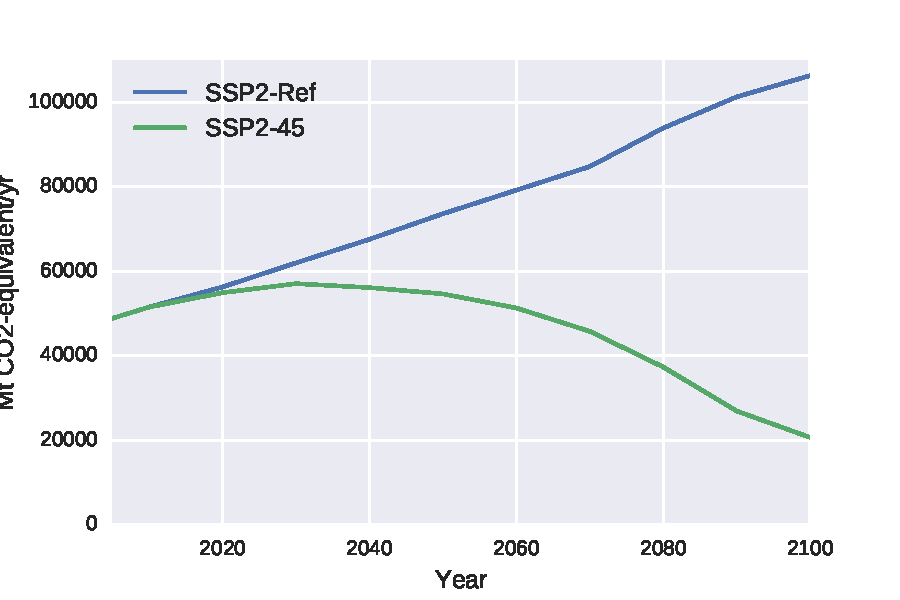
\includegraphics[width=\textwidth]{results_kyoto.pdf}
    \caption[]{
      \label{fig:kyoto}
      Unharmonized Kyoto gas emissions for SSP2-Ref, a scenario with generally
      increasing global emissions trends, and SSP2-45, a scenario with generally
      decreasing global emissions trends.  }
  \end{center}
\end{figure}


MESSAGE-GLOBIOM includes a representation of 11 distinct regions which can be
mapped directly to the 5-region definition used in the RCPs. Historical data is
taken from previously described LUC and anthropogenic sources, which comprise 10
separate pollutant and GHG species and 13 sectors shown in Table
\ref{tab:sp}. Therefore, a total of 1430 distinct trajectories were harmonized
for each scenario.

\begin{table}[]
  \centering
  \caption{Harmonized Species and Sectors}
  \label{tab:sp}
  \begin{tabular}{|l|l|}
    \hline
    \textbf{Emissions Species}        & \textbf{Sectors}                    \\
    \hline
    Black Carbon (BC)                 & Agricultural Waste Burning          \\
    Hexafluoroethane (C2F6)           & Agriculture                         \\
    Tetrafluoromethane (CF4)          & Aircraft                            \\
    Methane (CH4)                     & Energy Sector                       \\
    Carbon Dioxide (CO2)              & Forest Burning                      \\
    Carbon Monoxide (CO)              & Grassland Burning                   \\
    Hydrofluorocarbons (HFCs)         & Industrial Sector                   \\
    Nitrous Oxide (N2O)               & International Shipping              \\
    Ammonia (NH3)                     & Residential Commercial Other        \\
    Nitrogen Oxides (NOx)             & Solvents Production and Application \\
    Organic Carbon (OC)               & Transportation Sector               \\
    Sulfur Hexafluoride (SF6)         & Unharmonized                        \\
    Sulfur Oxides (SOx)               & Waste                               \\
    Volatile Organic Compounds (VOCs) &                                     \\
    \hline
  \end{tabular}
\end{table}

The effect of harmonization overrides is analyzed by harmonizing each scenario
first without and then with overrides. Of the 1430 trajectories, approximately
10\% were reported as a diagnostic (see Section \ref{sec:workflow}) of which 2\%
required the use of harmonization overrides after an initial investigation;
thus, 98\% of all trajectories were satisfactorily determined using the default
methods as chosen by the harmonization algorithm. Figure \ref{fig:nox} provides
one such example of a emissions species and sector in which all regions were
satisfactorily harmonized with the default methods. As can be seen, results with
and without overrides are identical.

\begin{figure}
  \begin{center}
    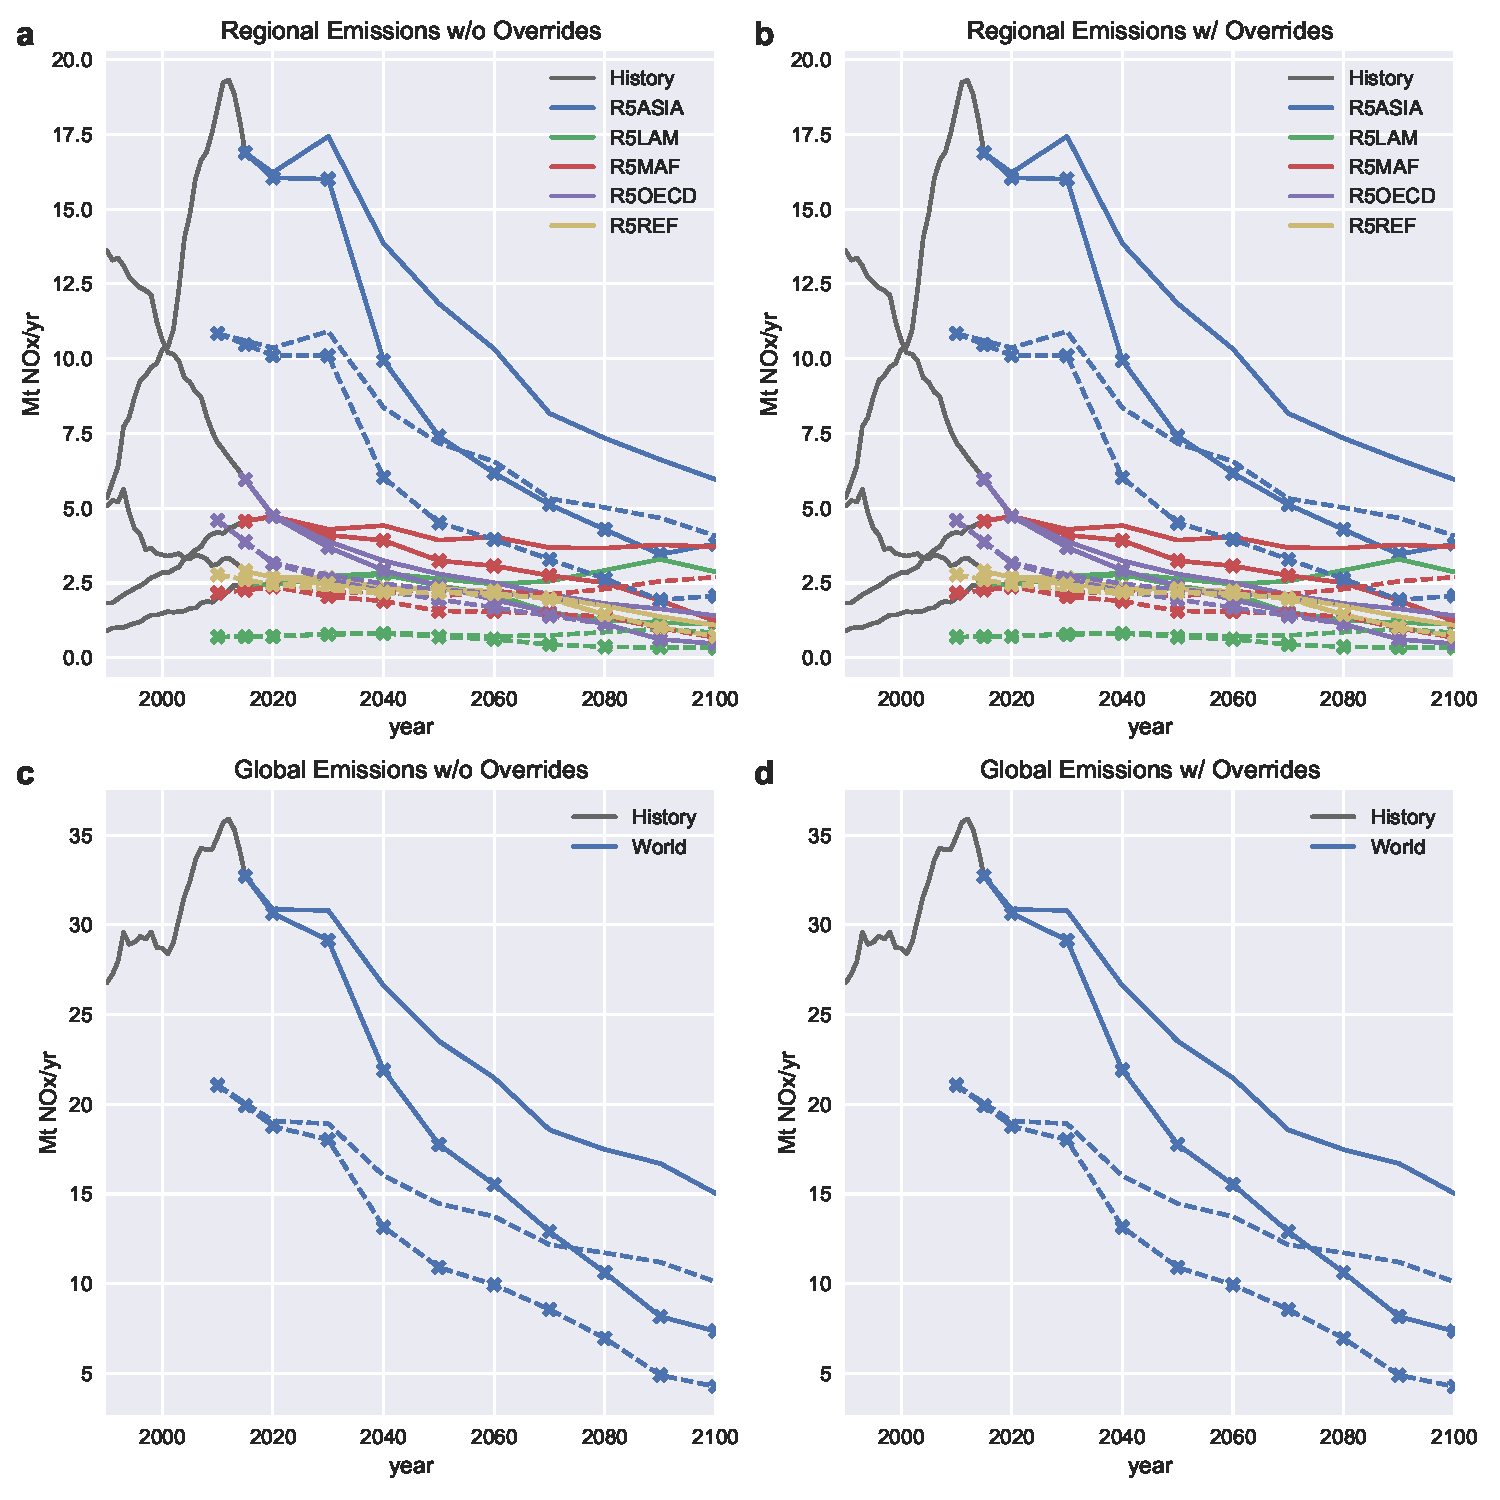
\includegraphics[width=\textwidth]{results_NOx_Energy_Sector.pdf}
    \caption[]{
      \label{fig:nox}
      NOx Energy Sector harmonized (solid lines) and unharmonized (dashed lines)
      trajectories for SSP2 and SSP2-45 are presented. SSP-45 is denoted with
      ``x'' markers. Panel \textbf{a} shows 5-Region trajectories for scenarios
      \textit{without} any overrides. Panel \textbf{b} shows 5-Region
      trajectories for scenarios \textit{with} overrides. Panels \textbf{c} and
      \textbf{d} show global trajectories without and with overrides,
      respectively.  }
  \end{center}
\end{figure}

The harmonization of emissions pathways is performed in order to accurately
represent an updated historical emissions trajectory while also maintaining
consistency with the original, unharmonized pathway. As such, when the default
methods as provided by the harmonization procedure distort or otherwise
sufficiently misrepresent the underlying unharmonized results, an override
method is required to be provided for the trajectory of the region, sector, and
species in question. Based on the 2\% of total trajectories required to be
overridden, two classifications were observed: regional trajectories whose
\textit{magnitude} was overly distorted and regional trajectories whose
\textit{shape} was overly distorted.

Figure \ref{fig:co} presents a case in which the magnitude of a trajectory is
distorted. A large discrepancy ($\sim$300\% relative difference) is
observed in the harmonization year for carbon monoxide (CO) emissions in the
industrial sector specifically for the South Asia (SAS) MESSAGE-GLOBIOM region,
which comprises most of the Asian subcontinent. The default method chosen
(\code{constant_ratio}) maintains model trends for the region; however, overall
model results are distorted. By applying a \code{constant_offset} override, the
regional trend and magnitude is maintained. With the new harmonization method
for the SAS region, the global trajectory for industrial CO also corresponds
more closely with the unharmonized trajectory.

\begin{figure}
  \begin{center}
    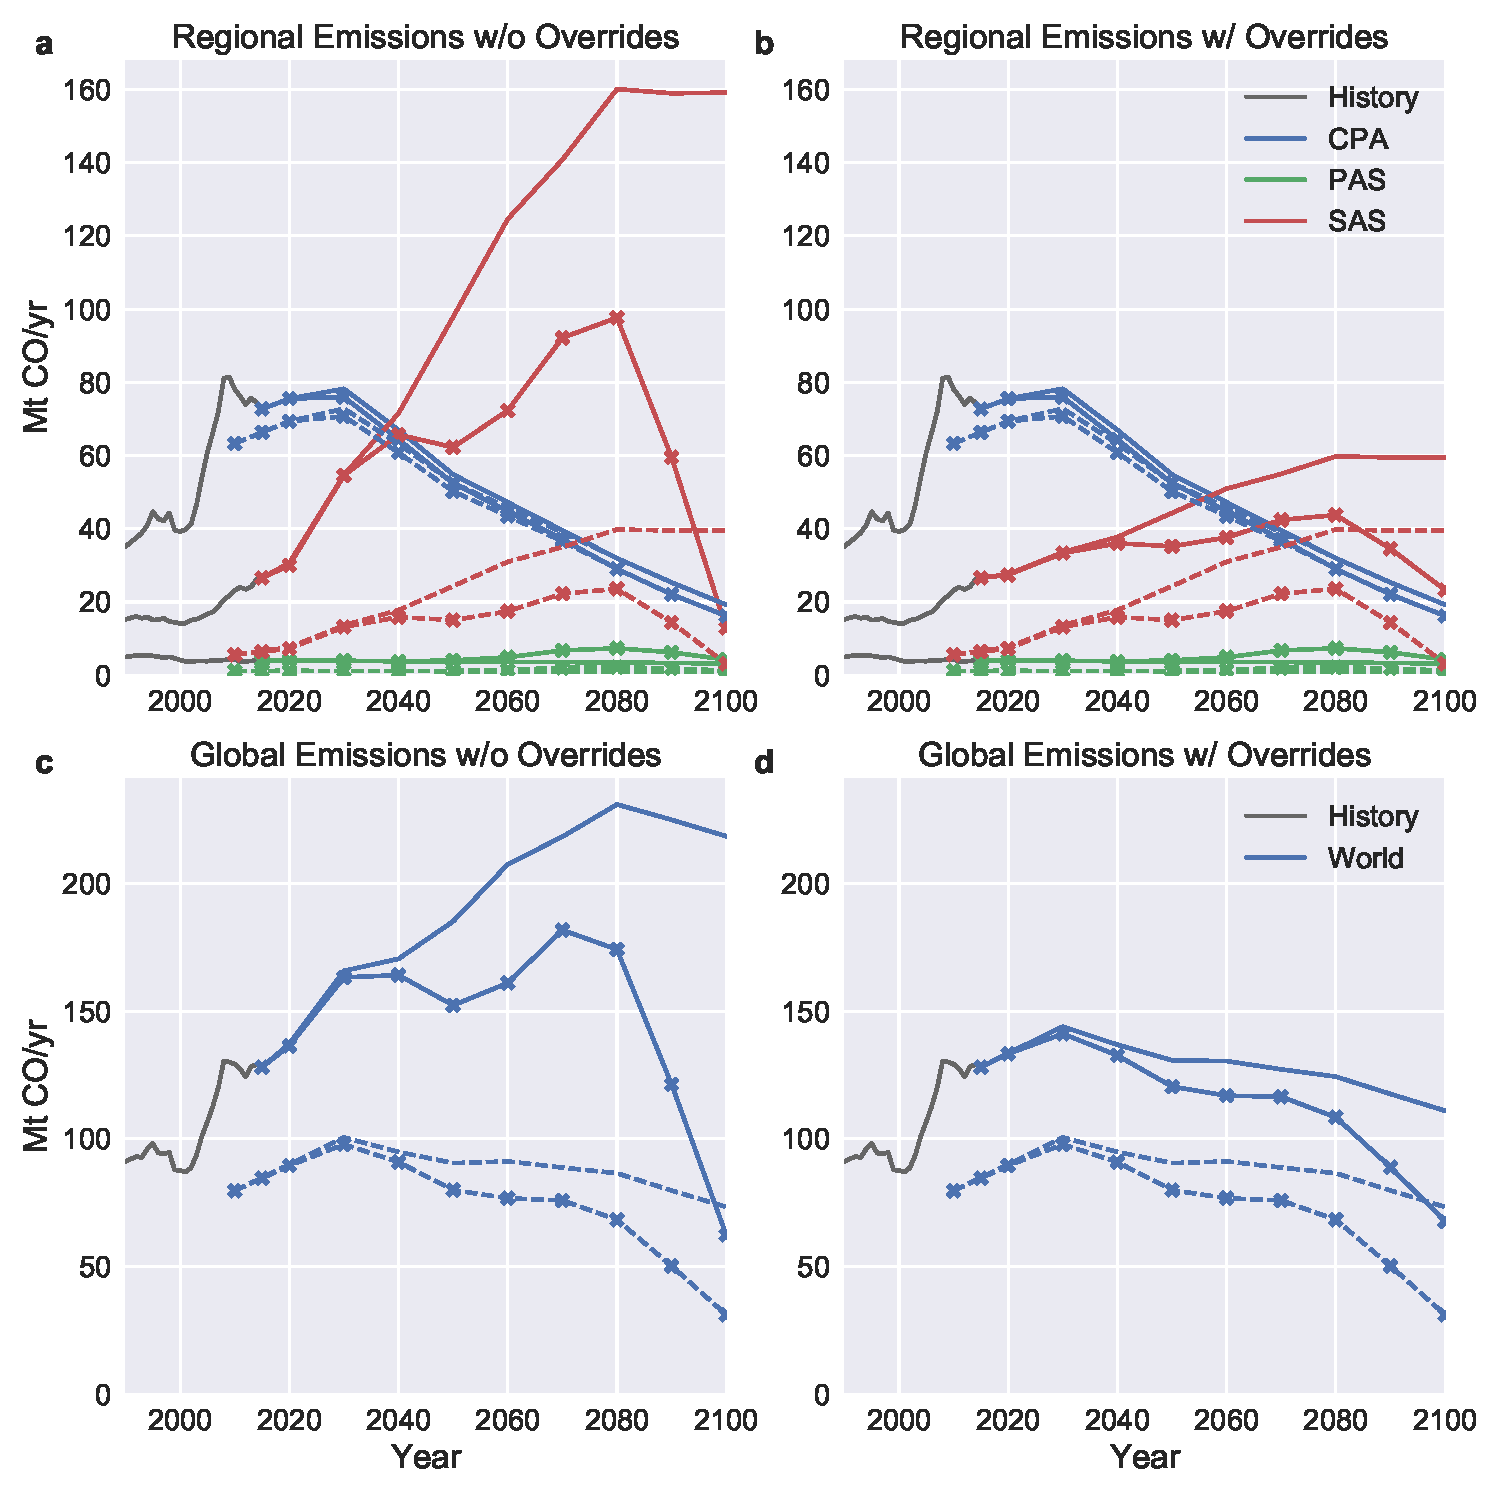
\includegraphics[width=\textwidth]{results_CO_Industrial_Sector.pdf}
    \caption[]{
      \label{fig:co}
      CO Industrial Sector harmonized and unharmonized emissions are presented
      for SSP2 and SSP2-45 scenarios. Scenarios as denoted identically to Figure
      \ref{fig:nox}. Panels \textbf{a} and \textbf{b} show harmonized and
      overridden-harmonized (respectively) regional trajectories for the 3
      MESSAGE-GLOBIOM regions that comprise the R5ASIA region: Centrally Planned
      Asia (CPA), Other Pacific Asia (PAS), and South Asia (SAS). Notably, the
      SAS regional trajectory displays a distorted trajectory due to the
      harmonization-year difference between history and model results in both
      scenarios. The distortion is large enough to affect global results, as
      shown in Panels \textbf{c} and \textbf{d}.  
}
  \end{center}
\end{figure}

In certain circumstances, the application of the default harmonization methods
can affect not only the magnitude but also the shape of regional
trajectories. Figure \ref{fig:nh3} shows an example case of emissions
trajectories for ammonia (NH3) from the agriculture sector in Asia. Again, the
SAS region shows a large discrepancy in the harmonization year ($>$150\% in
this case). The resulting trajectory harmonized with the default method
(\code{constant_ratio}) provides a large increase after 2080 in the SSP2
reference scenario. Notably, the SSP2-45 scenario is not affected to the same
degree. While this distortion changes the magnitude of the SAS trajectory, it
largely affects the post-2080 shape of the global trajectory (see Figure
\ref{fig:nh3}, panel \textbf{c}). By using a \code{constant_offset} method as an
override, this distortion is addressed and more accurately reflects unharmonized
results both in the SAS region and global results for agricultural ammonia
emissions.

\begin{figure}
  \begin{center}
    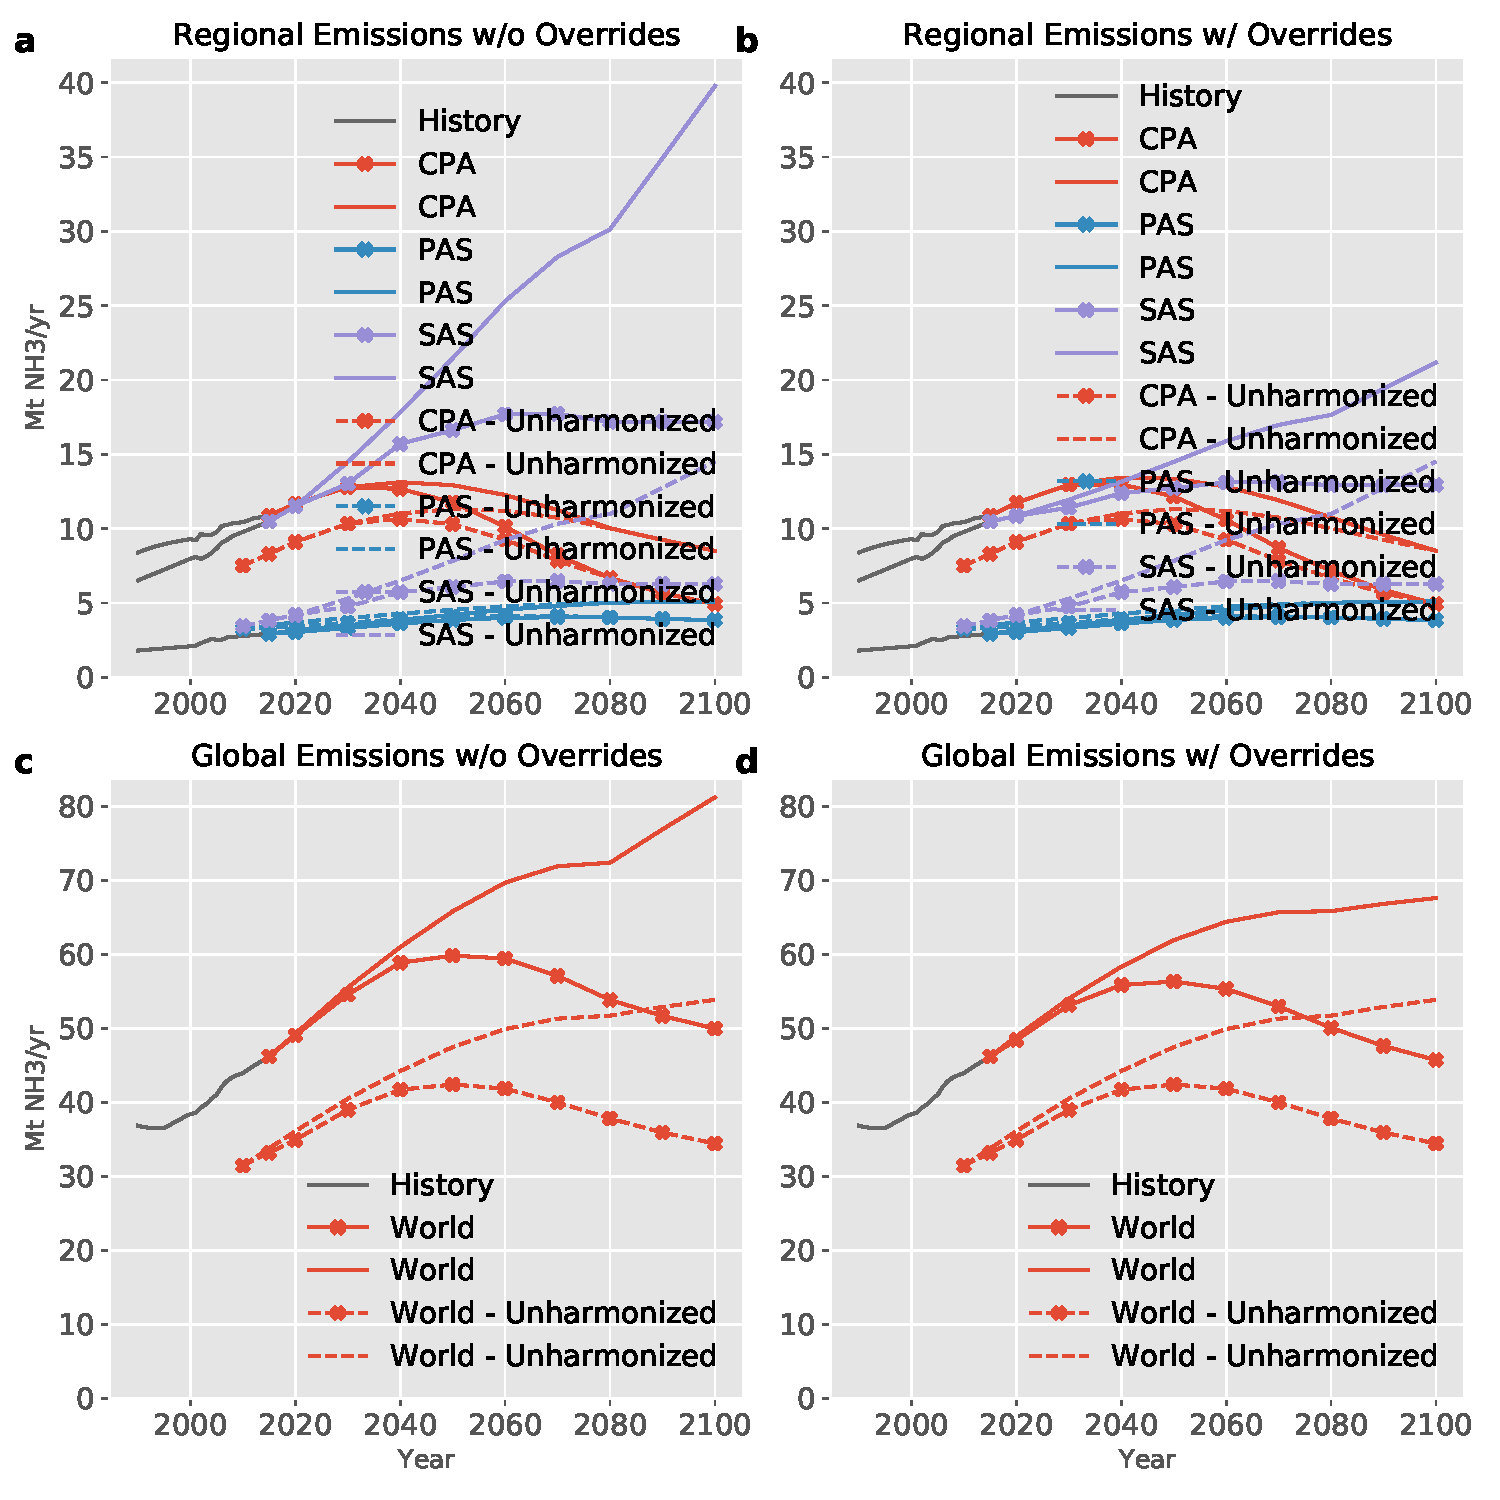
\includegraphics[width=\textwidth]{results_NH3_Agriculture.pdf}
    \caption[]{
      \label{fig:nh3}
      NH3 agricultural harmonized and unharmonized emissions are presented for
      SSP2 and SSP2-45 scenarios. Scenarios and panel layouts are identical to
      Figure \ref{fig:co}. In this case, the SAS trajectory again shows not only
      a magnitude distortion, but also a shape distortion at the tail of the
      trajectory. Additionally, global trajectories are greatly affected by the
      harmonization method choice (there is $\sim$20 percent relative difference
      between trajectories in the reference scenario in 2100). Override methods
      have been applied to correct the distortion.  }
  \end{center}
\end{figure}




